\section{RISC1-5: von Neumann Implementation}
\label{ch:von}
The presented Harvard Architecture uses separate memories for program and data. The advantage
is that instruction fetch and data execution can proceed concurrently. It was the revolutionary idea
of John von Neumann to merge the two. This made it possible to treat program code as data and to
perform operations on it. This was, for example, used for adding an array of numbers stored in
consecutive memory cells, typically performed by a tight program loop. Before each iteration, the
address of the instruction fetching the value to be added is incremented by 1.

This trick was made redundant by the later addition of index registers. Now computed values would
automatically be added to the constant in the instruction to form the effective address. In general,
modification of program code during execution proved to be a technique loaded with pitfalls, and it
is now virtually extinct. However, on a larger scale, loading of a (new) program is also based on
von Neumann’s concept of shared program and data memory, a feature without which computers are
unthinkable. Yet, the Harvard architecture is still used in applications, where the computer always
executes the same program. This is mostly the case in embedded applications for sensing data or
controlling machinery. Its advantage is a gain in speed, because program and data memories are
accessed concurrently.

\subsection{RISC1: Using large SRAM}
\label{sec:sram}
Before proceeding to a conversion of our RISC to the von Neumann scheme, we show the replacement of
the small 2KB BRAM for data storage by the large 1 MB SRAM. This large memory is not part of the
FPGA chip, but resides outside the FPGA on the Spartan-3 board. This necessitates that also the
environment of the RISC be adapted. We start by showing the changes necessary in the processor
circuit, rather than re-listing the entire circuit, and we start with the processor itself.

First of all, the address signals are doubled from 12 to 24 bits, the output $adr$ is widened from 5
to 20 bits.
\begin{verbatim}
  output[19:0] adr;
  adr = B[19:0] + off;
\end{verbatim}

The data BRAM $dm$ is removed, and with it the following signals:
\begin{verbatim}
  dmadr, dmwr, dmin, dmout, ioenb
\end{verbatim}

Connection to the SRAM is through the module’s interface (header), and thus the separation of
memory access and external device access is made in the environment (RISC1Top) rather than the
processor module. The signals $iowr$ and ford are now simply $wr$, $rd$.

So far, the changes are all removals resulting in simplifications. Memory access will now occur via
the environment like access to external devices, and the selector between memory and devices is
therefore moved to the environment. Hence, it is the environment that receives the extensions. This
is so, because the SRAM is external to the FPGA, and access via the FPGA’s pins can only be
specified in a top module. They appear in its parameter list:
\begin{verbatim}
  module RISC1Top( ...
    output SRce0, SRce1, SRwe, SRoe,
    output[ 3:0] SRbe,
    output[23:0] SRadr,
    inout [31:0] SRdat):
\end{verbatim}

The new declarations are
\begin{verbatim}
  wire[19:0] adr;
  wire[17:0] iowadr; // word address
  wire       rd, wr, ioenb;
  wire[31:0] inbus, inbusO, outbus;

  RISC1 riscx(.clk(clk), .rst(rst), .rd(rd),
              .wr(wr), .adr(adr),
              .inbus(inbus), .outbus(outbus)):
\end{verbatim}

The new signals (wires) obtain the following values:
\begin{verbatim}
  assign iowadr = adr[ 5:2];
  assign ioenb = (adr[23:6] == 18'h3FFFF):
  assign inbus = ~ioenb ? inbuso :
         ((iowadr == 0) ? cnt :
          (iowadr == 1) ? swi :
          (iowadr == 2) ? {24'bO, dataRx} :
          (iowadr == 3) ? {30'bO, rdyTx, rdyRx} : 0);
 
  assign SRce0 = 1'b0;
  assign SRce1 = 1'b0;
  assign SRwe = ~wr | clk;
  assign SRoe = ~rd;
  assign SRbe = 4'b0;
  assign SRadr = adr[19:2]:
 
  genvar i;
  generate             // tri-state buffer for SRAM
    for (i = 0; i < 32; i = i+1)
    begin: bufblock
      IOBUF SRbuf(.I(outbus[i]), .O(inbus0[i]),
                  .IO(SRdat[i]), .T(~wr)):
    end
  endgenerate
\end{verbatim}

The last paragraph specifies the tri-state buffer SAbuf. It is required, because the SRAM is
connected with the FPGA by a single, bi-directional bus SAdat. The circuits are shown
schematically in Figure \ref{fig:conn}.
\begin{figure}[h!]
  \centering
  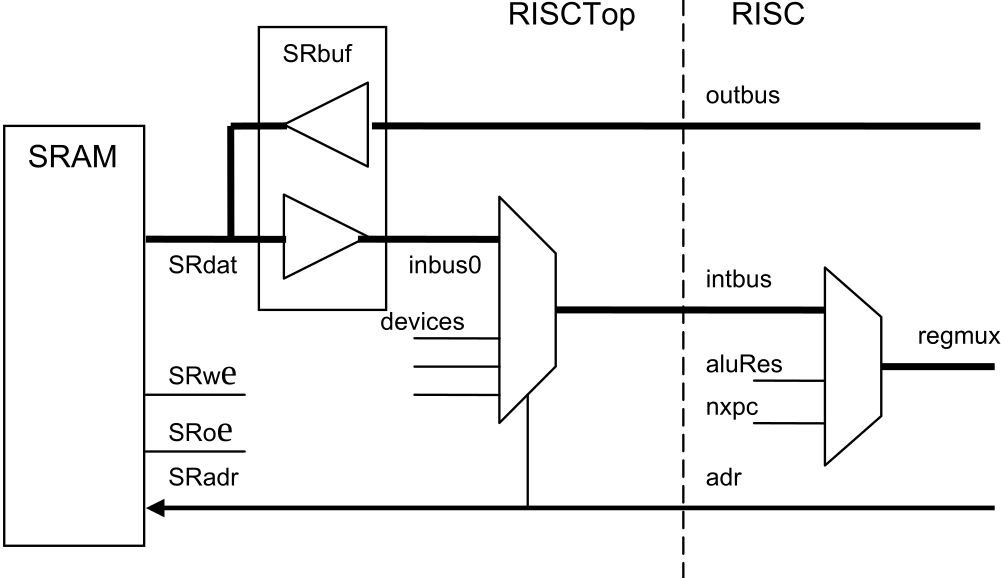
\includegraphics[width=.9\textwidth]{i/d.png}
  \caption{Connections between processor and SRAM}
  \label{fig:conn}
\end{figure}

The write strobe $wr$ determines the direction of the tri-state buffer. An absolutely essential
detail is that the write strobe be ored with the clock signal ($~wr | clk$). This is to activate
writing only in the 2nd half of the clock period. The SRAM is a combinational circuit, and writing
must wait until the address lines are stable, which is the case in the 2nd half of the cycle. The
various enable signals $ce0$, $ce1$, are all active (low). (Note that like in RISC0 we deal with
word transfers only, without byte selections. The least 2 address bits are ignored)

As an aside, we note that the SRAM is fast enough and is without a register at data output. This
makes a stall cycle unnecessary, again simplifying the processor. The clock rate is 35 MHz.

\subsection{RISC2: SRAM for both program and data}
We are now in a position to unite program and data memories following the concept of von Neumann.
There is practically no change in the top module, except that inbus0 is also brought to the
interface. It lets instructions bypass the multiplexer for input from external devices. Let us
consider the evolution of the processor.

First we note the widening of $PC$ (and $pcmux$ and $nxpc$) from 12 to 24 bits. Because instructions
are always 4 bytes long, their address is always a multiple of 4. This concerns the declarations
\begin{verbatim}
  output[23:0] adr;
  reg   [21:0] PC;
  wire  [21:0] pcmux, nxpc;
\end{verbatim}

In addition, the following changes are necessary:
\begin{verbatim}
  regmux =... (BR & v) ? {8'bO,nxpc,2'b0} : aluRes;
  pcomux =... (BR & cond & ~u) ? CO[23:2] : nxpc;
\end{verbatim}

When using the on-chip BRAM for PM, the IR is contained within the RAM. Its output $pmout$ is a
register. This is not so for the SRAM, and therefore a register has to be declared explicitly. We
call it $IR$.
\begin{verbatim}
  reg [31:0] IR;
  wire[31:0] ins;
  ins = IR;
  IR <= codebus;
\end{verbatim}

But this is only part of the story. We need to review the entire fetch/execute mechanism. Every
instruction is first fetched from memory into the IR. It is interpreted (executed) in the
\emph{next} cycle. In order to double speed, the instruction flow is pipelined: While an instruction
is executed, the next instruction is fetched. This works fine in the case of the Harvard
architecture. It also works for RIs in a von Neumann architecture, but not for MIs, because a data
access would interfere with the fetching of the next instruction. Therefore, a stall cycle must be
introduced for MIs, loads as well as stores. We let the $stall$ signal indicate, whether an
instruction fetch or a data access cycle is in progress. In the former case, the address is $pcmux$,
while in the latter it is $B + off$ (see Figure \ref{fig:smi}). The clock frequency had to be
reduced from 35 to 25 MHz.
\begin{verbatim}
  assign stall = stallL | stallM | stallD;
  assign stallL = (LDW | STW) & ~stall1;
 
  assign adr = stall ? B[23:0] + {4'b0O, off}
                     : {pcmux, 2'b00};
  assign wr = STW & ~stall1;
  assign rd = ~wr;
 
  regwr = ccwr | (LDW & ~stall1);
\end{verbatim}
\begin{figure}[h!]
  \centering
  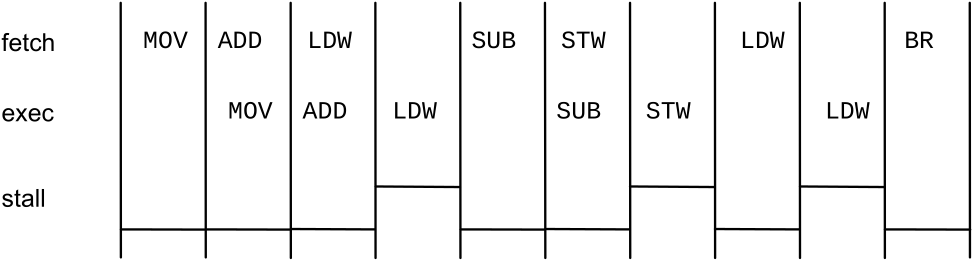
\includegraphics[width=.9\textwidth]{i/e.png}
  \caption{Stalling memory instructions}
  \label{fig:smi}
\end{figure}

There remains the (nasty) problem of how to load a program into the SRAM. The Xilinx loader always
loads a bit-stream into BRAM. In our case this is a boot loader for moving compiled code into the
SRAM. This implies that transfer of control from BRAM to SRAM must occur after the boot loading.
Of course we wish to use the RISC itself to execute the boot loader. For this purpose, we map the
BRAM (2K) onto SRAM, actually to its high end. $PMsel$ determines the memory from which instructions
are read.

The starting address on reset is now changed from 0 to $StartAdr$. The transfer of control after
boot loading is achieved by a branch to 0.
\begin{verbatim}
  reg PMsel;
 
  StartAdr = 22'h3FF800;
  IRBuf <= stall ? IRBuf : codebus;
  PMsel <= ~rst | (pcmux[18:11] == 8'hFF;
  ins = PMsel ? pmout: IR;
\end{verbatim}

\subsection{RISC3: Implementing byte-access}
The FPGA’s BRAMs are arrays of words, not bytes. We have therefore refrained from implementing
direct access to bytes. (of course bytes can be extracted and inserted by mask and rotate
instructions). Here we show how to provide byte-access in an efficient way which is possible,
because the SRAM allows to store individual bytes, although basically it is also word-oriented.
(In fact the SRAM of the Spartan board consists of 2 16-bit memory chips, and hence it might be
called \emph{half-word oriented}). The SRAM provides 4 write-enable signals, one for each byte in
a word. By generating these signals from the low 2 bits of the address, individual bytes can be
stored without affecting the other 3 bytes. Reading of a byte, however, always involves the reading
of the word containing it, and then shifting and masking the byte desired.

The only addition to the processor interface is the signal $ben$ (byte enable) derived from the
modifier bit $v$ in MIs.

For byte-wise reading, multiplexers are inserted into the input path. We rename the IOBuf’s output
from $inbus$ to $inbus0$, and redefine $inbus$ as
\begin{verbatim}
  inbusL = (~ben | a0) ? inbus[ 7: 0] :
                   a1  ? inbus[15: 8] :
                   a2  ? inbus[23:16] :
                         inbus[31:24];
  inbusH = ~ben ? inbus[31:8] : 24'bO;
  inbus = {inbusH, inbusL}:
 
  a0 = ~adr[1] & ~adr[0];
  a1 = ~adr[1] &  adr[0];
  a2 =  adr[1] & ~adr[0];
  a3 =  adr[1] &  adr[0];
\end{verbatim}

For byte-access writing, multiplexers need be inserted in the output path.
\begin{verbatim}
  assign obB0 = A|7:0];
  assign obB1 = ben & a1 ? A[7:0] : A[15: 8];
  assign obB2 = ben & a2 ? A[7:0] : A[23:16];
  assign obB3 = ben & a3 ? A[7:0] : A[31:24];
  assign outbus = {obB3, obB2, obB1, obB0};
\end{verbatim}

The various chip- and byte-enable signals are defined as (see also \ref{sec:sram}):
\begin{verbatim}
  SRced = be &  adr[1];
  SRce1 = be & ~adr[1];
  SRbe0 = be &  adr[0]:
  SRbe1 = be & ~adr[0];
  SRbe[2] = {SRce1, SRce0, SRbe1, SRbeO}:
  SRadr = adr[19:2];
\end{verbatim}

\subsection{Interrupts}
The last facility to be added is for interrupts. It was first introduced in computers around 1960.
The principal motivation was avoiding the need for distinct, small processors to handle small,
peripheral task, such as the acceptance of input data and of buffering them, before the actual
computing process was ready to accept them. Instead, the main process was to be interrupted, i.e.
the processor was to be borrowed (for a short time) to handle the request, and thereafter to be
returned to its interrupted task. Hence, the interrupt facility had a purely economical motivation.

One might assume that in the era of unbounded computing resources those small processes would
no longer have to share a processor, but would be represented by programs on separate, distinct
processors such as microcontrollers. This is partly happening. However, the interrupt is such a
convenient feature for economizing hardware that it continues to persist. It is indeed, as will be
seen shortly, very cheap to implement — at least in its basic form.

One should consider the effects of an interrupt evoked by an external signal as if a procedure call
had been inserted at random in the current instruction sequence. This implies that not only the call
instruction is executed, but also that the entire state of the current computation be preserved and
recovered after ending the interrupt procedure. Different strategies for implementation differ
primarily by the techniques for saving the state. The simplest implementation saves, like a
procedure call, only the current PC (in an extra register), and leaves the rest to the interrupting
program, such as the saving of used registers to software. This is the cheapest solution for
hardware, but also the most time-consuming for software. At the other end of the spectrum lies
hardware saving all registers including stack pointers, or even providing multiple sets of registers
for interrupts, letting an interrupt handler look as a regular procedure. A further sophistication
lies in providing several, distinct interrupt signals, perhaps even with distinct priorities, or
even programmable priorities. There is no limit to complexification.

One addition, however, is mandatory, namely a state register indicating whether or not interrupts
are admitted ($intEnb$). For the programmer of interest is that we obtain 3 new instructions, one
for returning from an interrupt routine, and 2 for setting the enable state. They are all encoded
in the form of BIs with $u = 0$:
\begin{figure}[h!]
  \centering
  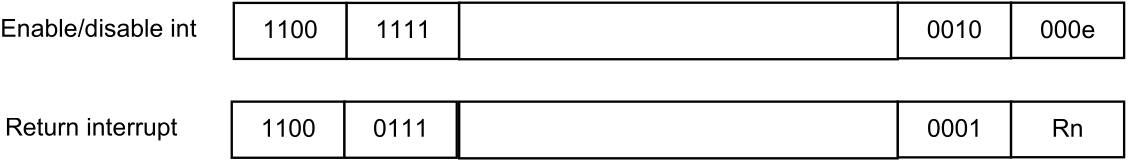
\includegraphics[width=.9\textwidth]{i/f.png}
  \caption{Special instructions for interrupt handling}
  \label{fig:ih}
\end{figure}

Following our credo for simplicity we here present a solution requiring the minimal effort on the side
of the hardware. This also lies in accord with the needs for teaching the concept. These are the
declarations of new variables:
\begin{verbatim}
  input      irq;    // INT request
  reg        irq1;   // edge detector
  reg        intMd, intEnb, intPnd;
                     // INT mode,enable,pending
  reg [25:0] SPC;    // saved PC & CC on INT
  wire[21:0] pcmux0;
  wire       intAck; // INT request enabled
  wire       nn, zz, cx, vv;     // CC
  wire       RTI;    // return from II
\end{verbatim}

When one of the $irq$ signals becomes high, an interrupt is pending. It causes $intAck$ to become
high, if interrupts are enabled ($intEnb$), the processor is not currently executing another
interrupt handler (\textasciitilde{}$intMd$), and the processor is not stalled. When $intAck$ is
high, the current PC is saved in the new SPC register, and $pcmux$ becomes 1, i.e. the next
instruction is read from address 4. At the same time, the condition bits are also saved (in
SPC[21:18]), and the processor enters the interrupt mode.
\begin{verbatim}
  intAck = intPnd & intEnb & ~intMd & ~stall;
  intPnd <= rst & ~intAck & ((~irq1 & irq) | intPnd);
  pcmux = ~rst ? 0: intAck ? 1 : pcmux0;
 
  N <= nn; Z <= zz; C <= cx; OV <= vv;
  SPC <= intAck ? {nn, zz, cx, vv, pcmux0} : SPC;
  intMd <= rst & ~RTI & (intAck0 | intAck1 | intMd);
\end{verbatim}

A ReTurn from Interrupt instruction (RTI) causes the next instruction address to be taken back from
SPC[21:0] and the condition bits from SPC[25:22]. Furthermore, the processor leaves the interrupt
mode.
\begin{figure}[h!]
  \centering
  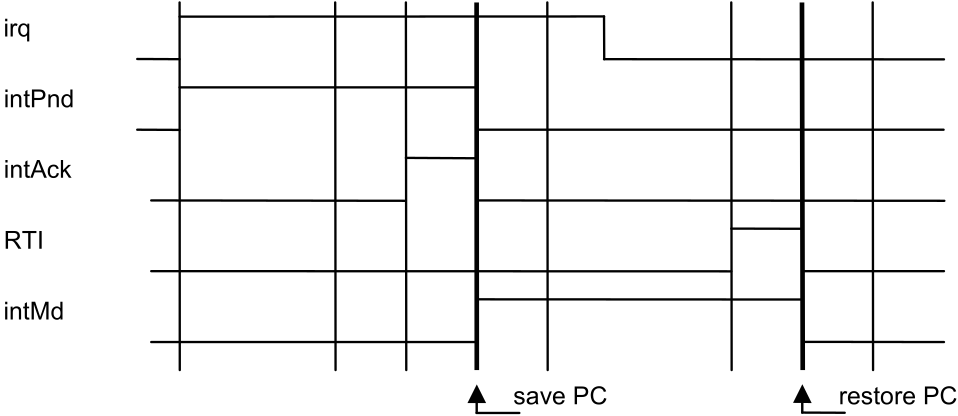
\includegraphics[width=.9\textwidth]{i/0.png}
  \caption{Interrupt signals}
  \label{fig:is}
\end{figure}
\begin{verbatim}
  RTI = p & q & ~u & IR[4];
  pcmux0 = stall ? PC : RTI ? SPC[21:0] : ...
  pcmux  = ~rsc ? StartAdr : intAck ? 1 : pcmux0;
 
  nn = RTI ? SPC[25] : ccwr ?  aluRes[31]       : N;
  zz = RTI ? SPC[24] : ccwr ? (aluRes[31:0]==0) : Z;
\end{verbatim}

The values for $cx$ and $vv$ are shown in the detailed program listings. The \emph{interrupt mode
instruction} copies $ins[0]$ into the $intEnb$ register, which is cleared on reset.
\begin{verbatim}
  intEnb <=                 ~rst ?     0  :
         (BR & ~u & ~v & ins[5]) ? ins[O] : intEnb;
\end{verbatim}

There is evidently very little additional circuitry due to the interrupt facility. However, this
solution requires that software saves and restored all registers used in an interrupt routine. Note
also that the interrupt routine must reset the external interrupt request. This typically is done by
a command to the respective device, effectively an acknowledge signal.

In order to generate an interrupt signal, the environment RISCTop is extended as follows. When
$cnt0$ reaches a limit, $cnt1$ is incremented and $irq$ is set to 1. This causes an interrupt every
millisecond, given a clock frequency of 25 MHz.
\begin{verbatim}
  assign limit = (cnt0 == 24999);
 
  always @(posedge clk) begin
    irq <= ~rst | (wr & ioenb & (iowadr==0))
          ? 0              : limit ? 1 : irq;
  end
\end{verbatim}
